\documentclass[a4paper,11pt]{ctexart}
\usepackage{srcltx,graphicx,float}
\usepackage{amsmath,amssymb,amsthm,mathrsfs}
\usepackage{algorithm}
\usepackage{color}
\usepackage{lscape}
\usepackage{psfrag}
\usepackage{diagbox}
\usepackage{bm}
\usepackage[hang]{subfigure}
\usepackage[colorlinks,linkcolor=black,anchorcolor=blue,citecolor=green]{hyperref}
\usepackage{geometry}
\usepackage{multirow}
\usepackage{array}
\newcommand{\PreserveBackslash}[1]{\let\temp=\\#1\let\\=\temp}
\newcolumntype{C}[1]{>{\PreserveBackslash\centering}p{#1}}
\newcolumntype{R}[1]{>{\PreserveBackslash\raggedleft}p{#1}}
\newcolumntype{L}[1]{>{\PreserveBackslash\raggedright}p{#1}}
\newcommand\bbN{\mathbb{N}}
\newcommand\diag{\mathrm{diag}}
\newcommand\tr{\mathrm{tr}}
\newcommand\dd{\mathrm{d}}
\renewcommand\div{\mathrm{div}}
\newcommand\bx{\boldsymbol{x}}
\newcommand\bF{\boldsymbol{F}}
\newcommand\bu{\boldsymbol{u}}
\newcommand\bn{\boldsymbol{n}}
\newcommand\bv{\boldsymbol{v}}
\newcommand\bU{\boldsymbol{U}}
\newcommand\bA{\boldsymbol{A}}
\newcommand\vecf{\boldsymbol{f}}
\newcommand\hatF{\hat{F}}
\newcommand\flux{\hat{F}_{j+1/2}}
\newcommand\diff{\mathrm{d}}
\newcommand\pd[2]{\dfrac{\partial {#1}}{\partial {#2}}}
\newcommand\od[2]{\dfrac{\dd {#1}}{\dd {#2}}}
\newcommand\abs[1]{\lvert #1 \rvert}
\newcommand\bbC{\mathbb{C}}
\newcommand\bbR{\mathbb{R}}
\geometry{left=2.5cm,right=2.5cm,top=2.5cm,bottom=2.5cm}
\graphicspath{{pictures/}}
\title{Octave学习}
\author{吴艺翀\quad1601110035\thanks{北京大学数学科学学院,科学与工程计算系,邮箱: {\tt wuyichongyt@sina.cn}}}
\begin{document}
\maketitle
\tableofcontents
\newpage
\section{Octave简介}
Octave是一款用于数值计算和绘图的软件,它属于GNU计划,因此是开源的。和MATLAB类似,它尤其精于矩阵运算,能够批量处理相关问题并很好的将数据可视化。它是一门基于C++的解释性语言,相比于编译性语言,转化为机器语言的速度更慢,但其代码功能实现上的优势弥补了这一缺陷,大大提高了有关工作的效率。\par
最初,Octave是作为一款本科生化学课程的辅助程序由Octave Levenspiel等人开发的,它的名字也由此而来。真正完整的发展是由John W.Eaton于1992年开始的,1993年1月4日公布第一个alpha版本,1994年2月17日1.0版本公布,目前的4.0.0版本于2015年5月29日公布。\par
Octave与MATLAB有着极大地相似性,事实上,在它的开发过程中就视与MATLAB的兼容性为一项要求,不兼容将被视作Bug。因此,Octave可以认为是在不侵权的前提下对MATLAB的软件“克隆”。那么,学习Octave的过程中,抓住它与MATLAB的异同是关键,尤其是对于有MATLAB基础的学习者来说。
\section{Octave的使用}
\subsection{安装及进入界面}
安装十分简单,在命令行中输入sudo apt-get install octave即可,安装的是4.0.0版本。值得一提的是从3.8.0版本开始,Octave支持图形用户界面(GUI),安装完毕后在命令行输入octave将自动进入GUI,若想在命令行界面中使用,应输入octave --no-gui.
启动后如下
\begin{figure}[H]
	\begin{center}
		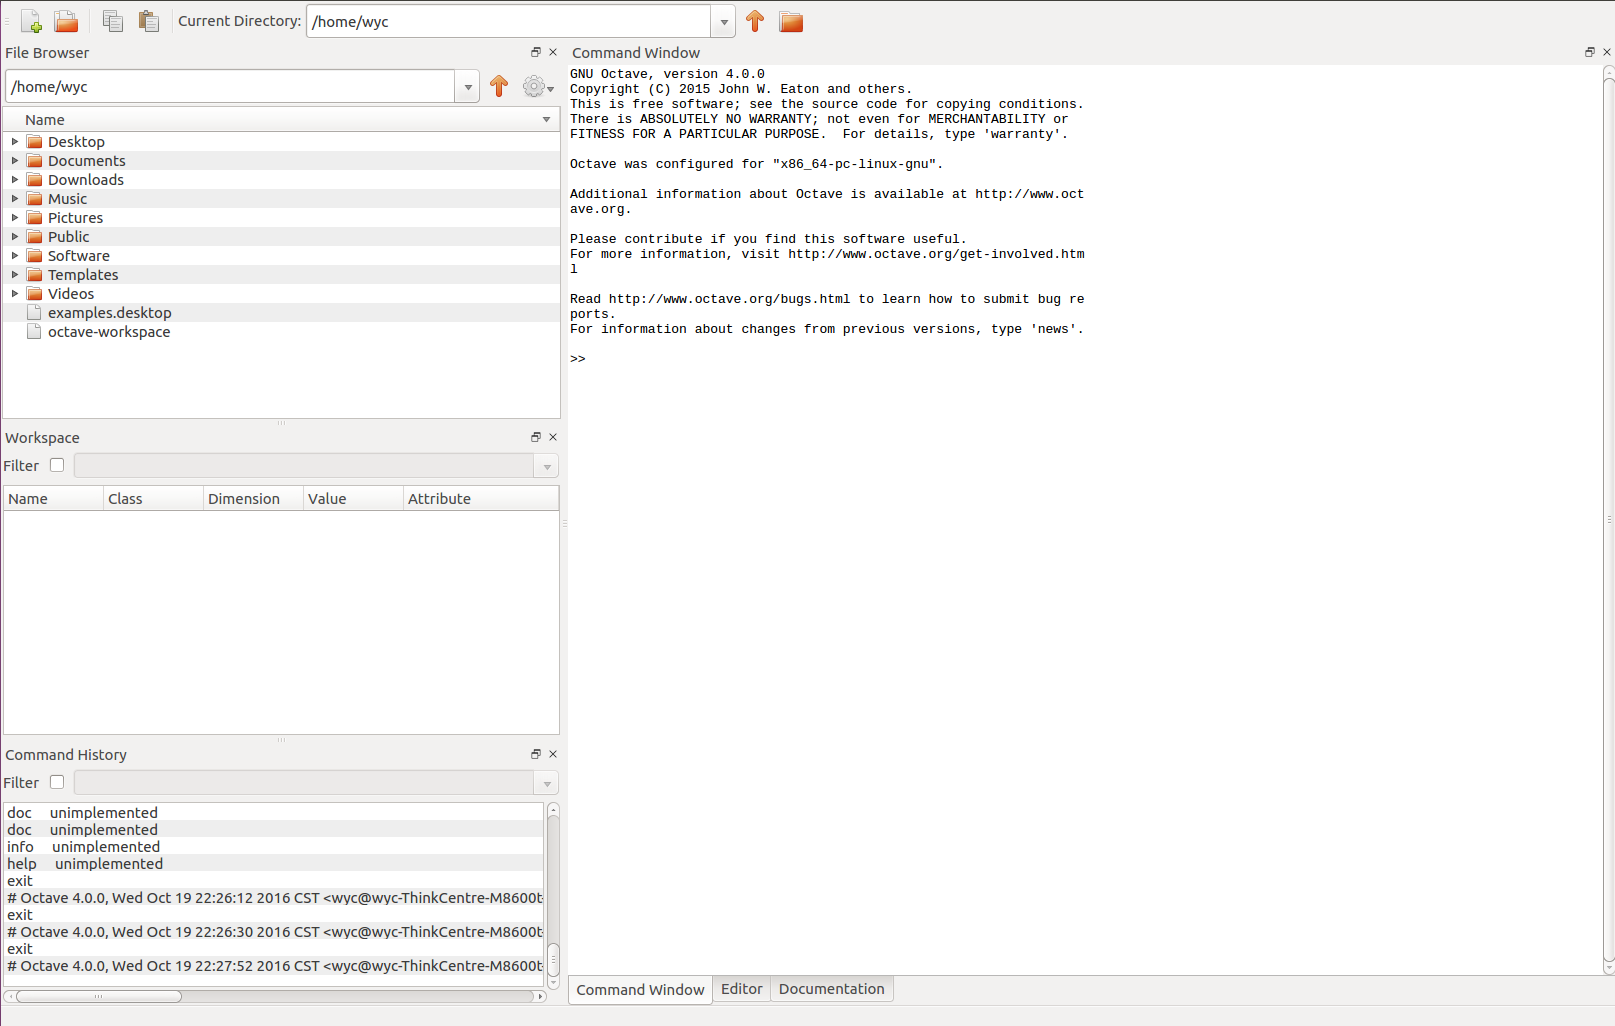
\includegraphics[width=.9\textwidth]{octave.png}
	\end{center}
	\caption{图形用户界面}
%	\label{fig:<+label+>}
\end{figure}
\begin{figure}[H]
	\begin{center}
		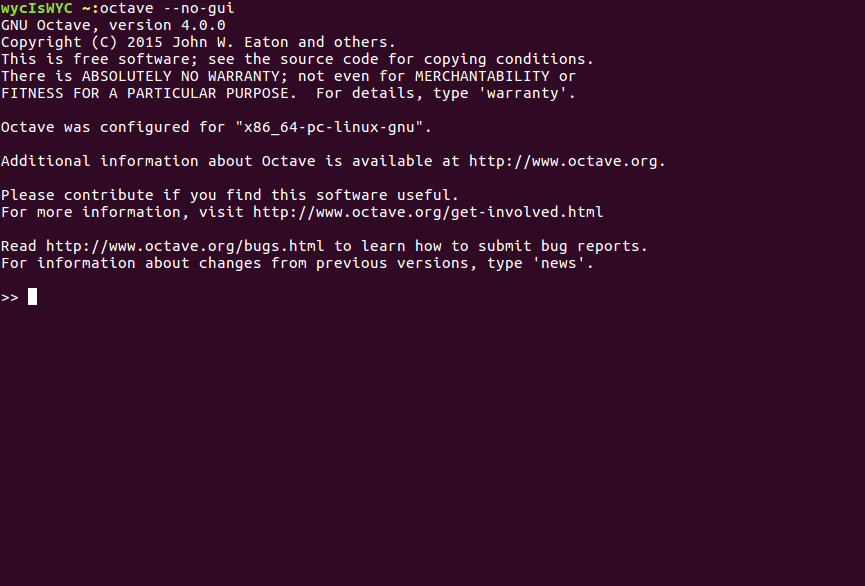
\includegraphics[width=.9\textwidth]{octave_no_gui.png}
	\end{center}
	\caption{命令行界面}
%	\label{fig:<+label+>}
\end{figure}


\subsection{简单计算}
Octave最简单的使用方式就是像使用计算器一样在命令提示符下输入相应的计算式,它能识别通常的计算表达式。各种计算符号的优先级与常规的一致,比如括号有最大优先级,其次为乘方,其次为乘除运算,最后为加减运算。
\begin{figure}[H]
	\begin{center}
		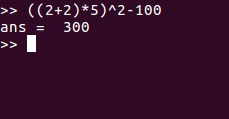
\includegraphics[width=.6\textwidth]{simplecal.png}
	\end{center}
	\caption{简单计算}
%	\label{fig:<+label+>}
\end{figure}
\subsection{分号和隐藏结果}
分号在通常的编程语言例如C++中被用来表示程序块或者单个语句的结束。然而在Octave中分号的作用并非如此。在之前的例子中,我们输入一个Octave命令结尾处没有加上分号,那么Octave会将语句执行的结果随即显示出来。而如果我们在一行语句的末尾添上l了分号,Octave将不会显出相应的结果。这样做有时更利于我们观察运行情况,而不会被中间的一些无关紧要的数据所干扰。
\subsection{内建函数}
除了这些最基本的计算符,Octave还提供了一系列的常用数学函数。通过调用这些函数,可以方便有效的完成我们的工作。与C++调用函数一样,Octave通过输入函数名和括号中的输入参数来调用函数,例如计算$1.2\sin(40^{\circ}+\ln(2.4^2))$\\                       
\begin{figure}[H]
	\begin{center}
		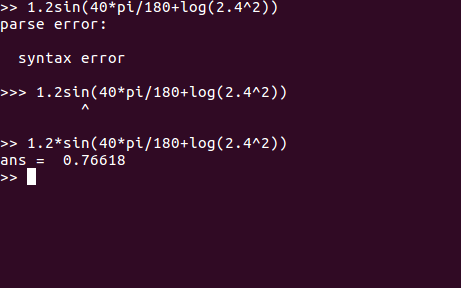
\includegraphics[width=.9\textwidth]{sinlog.png}
	\end{center}
	\caption{内建函数的使用}
%	\label{fig:<+label+>}
\end{figure}
在刚才的例子中,需要注意的是:在计算表达式中一个明确的乘号是必不可少的,比如在 1.2 和$\sin$间,这和我们手写的习惯不同。下面给出一些常用的基本函数
\begin{table}[H]
	\centering
	\begin{tabular}{L{6cm}L{5cm}}
		\hline
cos & 余弦函数 (弧度制)				\\
sin  &正弦函数 (弧度制)	\\
tan & 正切函数 (弧度制)	\\
exp & 指数函数 (e x )	\\
log & 以 e 为底的指数函数	\\
log10 & 以 10 为底的指数函数	\\
sinh & 双曲正弦函数	\\
tanh & 双曲正切函数	\\
cosh & 双曲余弦函数	\\
acos & 反余弦函数	\\
acosh & 反双曲余弦函数	\\
asin & 反正弦函数	\\
asinh & 反双曲正弦函数	\\
atan & 反正切函数	\\
atan2 & 双参数形式的反正切函数 	\\
atanh & 反双曲正切函数	\\
abs & 绝对值函数 (复数取模)	\\
sign & 符号函数	\\
round & 四舍五入	\\
floor & 近似为比它小的最大整数	\\
ceil & 近似为比它大的最小整数	\\
fix & 向 0 方向近似	\\
rem & 求余数	\\
\hline
	\end{tabular}
	\caption{基本数学函数}
%	\label{tab:<+label+>}
\end{table}
\subsection{取消一个命令}
如果你发现输入的一个命令执行了很长的时间都没有结束,中止该程序的执行就变得又必要。你可以在当前命令行下输入Ctrl-C,程序将被中止并返回到命令提示界面。至于究竟是你程序自身的Bug还是其他原因导致命令的执行缓慢,就需要你去进一步探索。
\subsection{help}
Octave的功能十分强大,它有许多命令以及内建函数。想要一次性全部掌握是不太现实的。如果你刚接触某个命令或者函数,还不了解它的使用方式,Octave本身的帮助系统会很有用,它能让你第一时间清楚相关信息。例如我们想要知道函数sqrt的介绍,最基本的使用帮助系统的方式就是
\begin{figure}[H]
	\begin{center}
		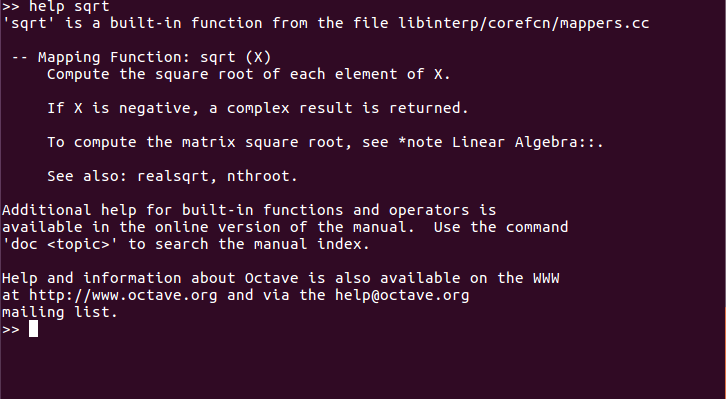
\includegraphics[width=.9\textwidth]{help.png}
	\end{center}
	\caption{help的使用}
%	\label{fig:<+label+>}
\end{figure}
这个函数比较简单,对于一些复杂的函数,通过help可以清晰的了解它的使用方法。\par
如果你不知道你需要的某个函数的具体名称,有个方法可以帮助你找到这样的函数是否存在。通过命令行输入help --list,Octave 将给出一个其帮助的主题列表.你可以从中找到你想要的功能。
\begin{figure}[H]
	\begin{center}
		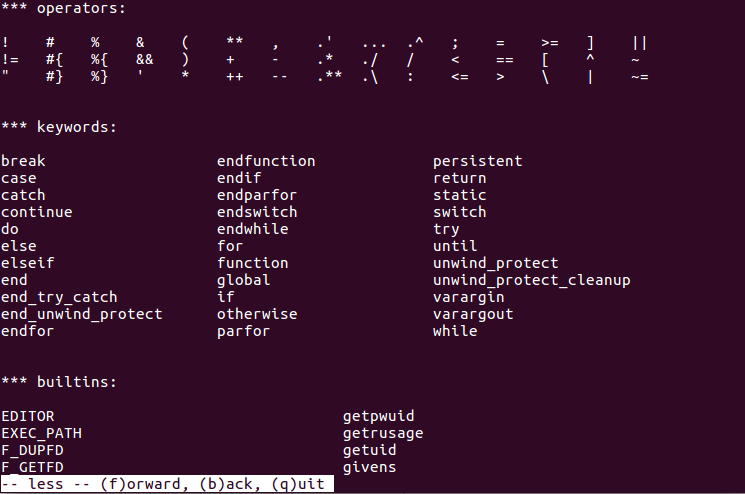
\includegraphics[width=.9\textwidth]{helplist.png}
	\end{center}
	\caption{help --list结果}
%	\label{fig:<+label+>}
\end{figure}
\newpage
\section{矩阵和向量}
要想在Octave中高效的进行计算,就得利用好它的矩阵运算机制。遇到问题时,尽量使用矩阵(向量也是矩阵)代替循环,这样可以节省大量运算。\par
\subsection{矩阵的构建}
\subsubsection{方括号}
构建矩阵的方法有很多。其中最直接简单的方法就是在一个方括号[ ]中给出其元素.在方括号中由空格或者逗号隔开的一组数据被定义为行向量; 而由分号或者回车隔开的一组数据被定义为列向量.
\begin{figure}[H]
	\begin{center}
		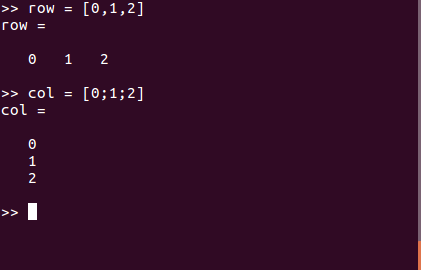
\includegraphics[width=.6\textwidth]{vector.png}
	\end{center}
%	\caption{<+caption text+>}
%	\label{fig:<+label+>}
\end{figure}
\subsubsection{冒号}
冒号也是很重要的一个工具,在构建矩阵以及提取矩阵元素中都有着很大的作用。
\begin{figure}[H]
	\begin{center}
		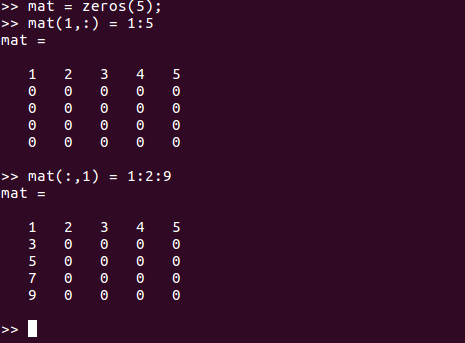
\includegraphics[width=.6\textwidth]{maohao.png}
	\end{center}
%	\caption{冒号的使用}
%	\label{fig:<+label+>}
\end{figure}
单独的一个冒号表示整行或整列;$a:b$表示一个以$a$为首项,1为公差,最后一项不大于$b$的等差数列(这是$a<b$的情况,反之类似);$a:b:c$表示以$a$为首项,$b$为公差,最后一项不大于$c$的等差数列。\par
一些常用的构建矩阵的方法如下
\begin{table}[H]
	\centering
	\begin{tabular}{ll}
		\hline
eye  &创建单位矩阵\\
zeros &创建全零矩阵\\
ones &创建全一矩阵\\
linspace(x1,x2,N)	& 创建一个$N$个元素的向量,均匀分布于$[x_1,x_2]$	\\
logspace(x1,x2,N)	& 创建一个$N$个元素的向量,指数分布与$[10^{x_1},10^{x_2}]$ \\
rand &创建随机数矩阵\\
diag &创建一个对角矩阵,或者提取一个矩阵的对角元\\
		\hline
	\end{tabular}
	\caption{矩阵的构建}
%	\label{tab:<+label+>}
\end{table}
\subsection{矩阵的操作}
矩阵中的元素通过括号 ()提取,而第一个元素的编号为 1, 而不是像 C 或者 C++ 那样从 0 开始.\par
在 C++ 中如果你想进行相同的计算,例如每个元素乘以 2, 你需要使用 for 循环来对每个元素操作。在 Octave 中虽然也可以使用 for 循环来实现,但是 Octave 本身由有简单的向量操作方式。
对于加减以及数乘运算,相应的就是向量各分量上的运算。而矩阵的乘法必须要求矩阵的形状相符合。另外,在运算符号前加一个.代表对应元素的运算。
\begin{figure}[H]
\begin{minipage}[t]{0.5\linewidth}
\centering
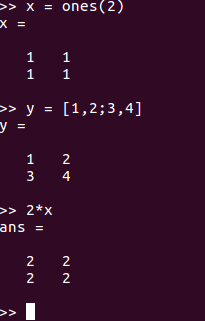
\includegraphics[width=.5\textwidth]{vector1.png}
%\caption{fig1}
%\label{fig:side:a}
\end{minipage}%
\begin{minipage}[t]{0.5\linewidth}
\centering
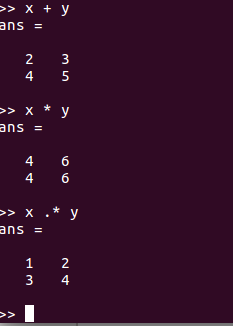
\includegraphics[width=.5\textwidth]{vector2.png}
%\caption{fig2}
%\label{fig:side:b}
\end{minipage}
\end{figure}
而除法$A/B$则代表着求解方程$XB=A$,这自然要求$B$可逆。矩阵转置则只需在矩阵后加上一个单引号。\par
一些常用的操作矩阵的方法如下
\begin{table}[H]
	\centering
	\begin{tabular}{L{4cm}l}
		\hline
inv &求矩阵逆矩阵\\
det &求矩阵特征值\\
trace &求矩阵的迹\\
eig &求矩阵的特征向量和特征值\\
rank &求矩阵的秩\\
null &求矩阵零空间的基\\
rref &对一个增广矩阵进行Gauss消去\\
lu &求矩阵的LU分解\\
qr &求矩阵的QR分解\\
svd &求矩阵的SVD分解\\
pinv &求矩阵的广义逆\\
		\hline
	\end{tabular}
	\caption{矩阵的操作}
%	\label{tab:<+label+>}
\end{table}
\newpage
\section{作图}
Octave的作图是通过调用开源软件GNUPLOT来实现的。
\subsection{基本绘图:plot}
最基本的2维画图命令是plot(x,y),其中x,y分别为横轴和纵轴数据。我们可以加上一些参数使线条样式更多样化
\begin{table}[H]
	\centering
	\begin{tabular}{L{4cm}L{2cm}}
		\hline
		颜色 & 点的类型\\
		\hline
		w 白色&. 点\\
		c 青色&o 圆圈\\
		r 红色&x x形\\
		g 绿色&* 星号\\
		b 蓝色&+ +号\\
		\hline
	\end{tabular}
	\caption{线条样式参数}
%	\label{tab:<+label+>}
\end{table}
\noindent 再之后,title,xlabel,ylabel分别为图片添加标题和xy轴名称
\begin{figure}[H]
	\begin{center}
		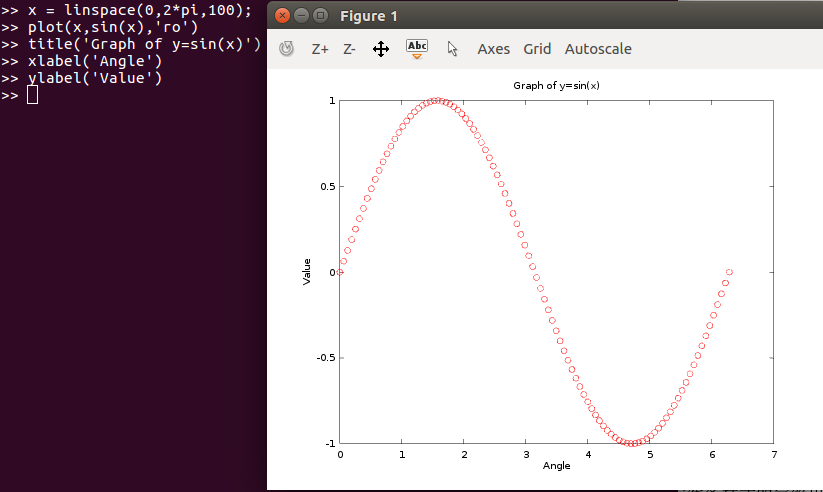
\includegraphics[width=.8\textwidth]{plotl.png}
	\end{center}
	\caption{plot基本操作}
%	\label{fig:<+label+>}
\end{figure}
\subsection{持续操作:hold on}
如果你想在当前图形下继续进行操作,你可以通过使用hold on命令来实现。使用该命令后,我们可以实现在同一幅图上呈现由多个plot命令绘制的线条。\par
而多幅图片可以通过figure命令来控制,在命令行中输入figure那么下一个plot命令将会在新创建的窗口中绘制(如果既不hold on也不figure,那么新的plot会取代之前的图形)。
\begin{figure}[H]
	\begin{center}
		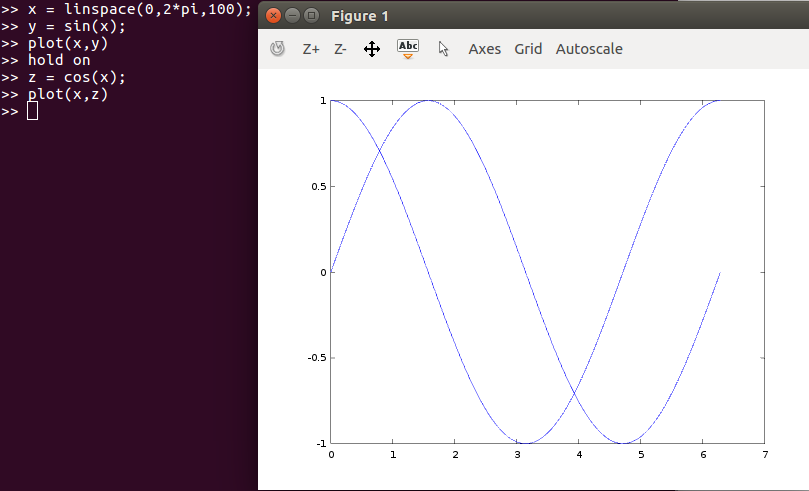
\includegraphics[width=.8\textwidth]{plot.png}
	\end{center}
	\caption{hold on指令}
%	\label{fig:<+label+>}
\end{figure}
\subsection{创建子图:subplot}
要在同一个窗口中创建多幅子图要通过subplot命令实现。该命令能够将窗口分离成一系列的子窗口,其基本语法为
$$\text{subplot(row,columns,num)}$$
其中num参数指定当前绘图在子窗口中的序号,序号按照从上到下,从左到右的次序递增。接下来用一个例子来说明subplot的应用
\begin{figure}[H]
	\begin{center}
		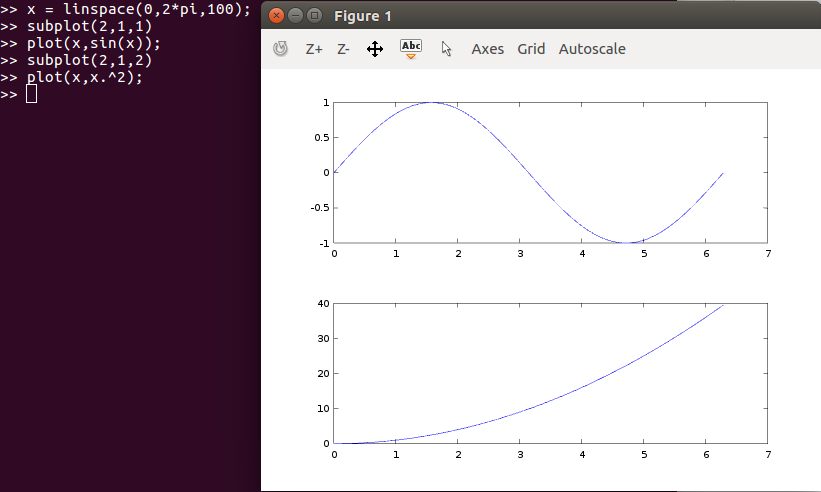
\includegraphics[width=.8\textwidth]{subplot.png}
	\end{center}
	\caption{subplot指令}
%	\label{fig:<+label+>}
\end{figure}
\subsection{3D绘图:plot3}
Octave同样可以进行3D数据的可视化,最简单的3D绘图实现是由plot3命令完成的,与plot命令类似,该命令通过接受输入的 x,y 和z轴的数据,绘制出点或者线。接下来的例子画出了一个螺旋线,使用参数式的函数
\begin{figure}[H]
	\begin{center}
		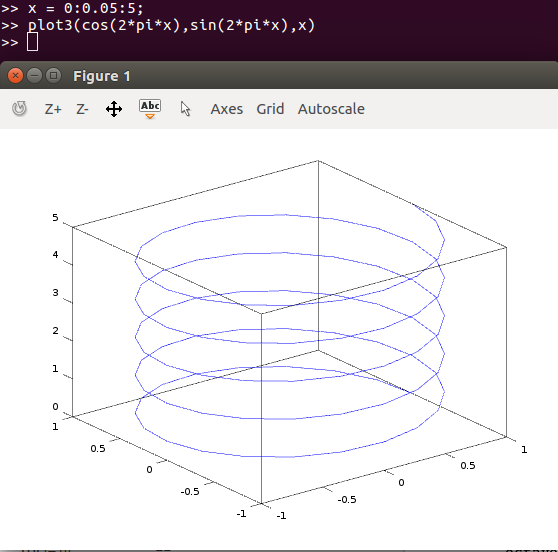
\includegraphics[width=.8\textwidth]{3dplot.png}
	\end{center}
	\caption{3D绘图}
%	\label{fig:<+label+>}
\end{figure}
\subsection{绘制曲面:meshgrid,surf}
除了三维的线与点之外,我们还需要绘制曲面。例如一个函数
$$z=f(x,y)=(x−3)^2−(y−2)^2,x\in[2,4],y\in[1,3]$$
为了绘制曲面,我们首先要生成xy平面上的网格,这通过meshgrid命令实现.之后求得对应网格上的函数值,利用surf指令生成曲面
\begin{figure}[H]
	\begin{center}
		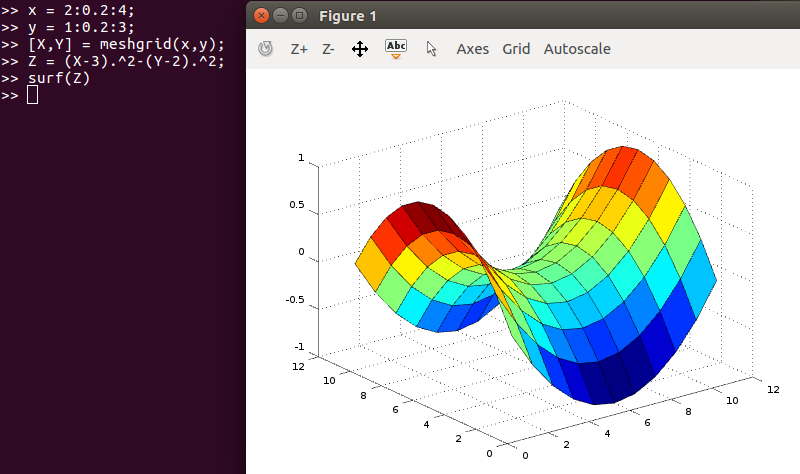
\includegraphics[width=.8\textwidth]{surf.png}
	\end{center}
	\caption{曲面的绘制}
%	\label{fig:<+label+>}
\end{figure}
\newpage
\section{脚本文件与函数}
如果你想实现的目标比较复杂,那么直接通过终端输入及修改指令会很不方便。你可以将这一系列的指令存入一个Octave脚本之中。
这种包含Octave指令的文本文件是Octave程序的基本形式。当你在Octave中执行这样的脚本的时候,其效果与将这些指令一行行输入Octave中是一样的。
而且当你对一系列要输入Octave的指令不是很拿的准的时候,在一个脚本中修改这些指令会比在Octave终端中重新调出及修改指令要简单方便许多。
Octave的脚本是普通的文本文件,它们需要一个.m的后缀。因此,它们被称为M文件。除去后缀的文件名部分是你在执行该命令时需要向Octave 终端输入的部分。\par
你可以在任何的文本编辑器(如,emacs,vim,notepad)中创建并编辑一个脚本文件。在Octave中输入命令edit将在新窗口中调出文本编辑器emacs。要运行某个脚本时,例如run.m,只需在相关路径下输入脚本名run即可。另外,$\%$后的一行语句代表注释,将被Octave解释器忽略。\par
Octave假定一个脚本文件的头几行注释是该脚本的描述,这几行注释也是你使用help命令时获得的信息,因此在你每个脚本的头几行写上有关该脚本的帮助信息是一个很好的习惯。
\begin{figure}[H]
	\begin{center}
		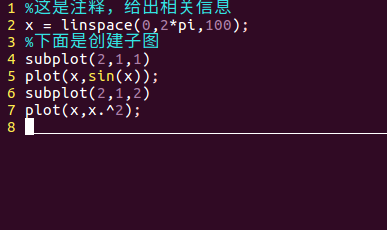
\includegraphics[width=.8\textwidth]{m.png}
	\end{center}
	\caption{脚本文件}
%	\label{fig:<+label+>}
\end{figure}
\subsection{控制语句}
复杂的脚本文件通常需要用到各种各样的控制语句。与常用的语言类似,Octave也提供了标准的控制语句。需要再次提醒的是,尽量用矩阵形式的计算代替循环语句,这有利于提高运行效率。
\subsubsection{if...else语句}
如果你想在程序中有条件的执行一些操作,就需要if这样的条件执行语句.Octave中if语句的一般用法是\\
if expression\\
\indent statements\\
elseif expression\\
\indent statements
\subsubsection{for语句}
for循环是编程语言中另一个常用的结构,它将一定次数的重复执行一段代码。虽然我们多次强调在Octave中你应该多使用矩阵的计算而不是for循环,因为通常for循环会慢很多。然而有的时候for循环是不可避免的。该语句的语法是\\
for variable=vector\\
\indent statements\\
end
\subsubsection{while语句}
如果你不知道需要执行多少次循环,而是知道当某条件满足时结束循环。Octave中的while语句能实现该功能\\
while expression\\
\indent statements\\
end
\subsection{函数}
通过脚本文件,再加上内建函数的帮助,我们能实现一些目标。但是当遇到要多次重复用到某一段代码的功能时,就需要用户自定义函数。自定义函数能够让你在命令行、其他函数中和脚本中调用,使你的代码更加简介清晰。\par
在Octave函数中参数是通过值传递的而不是通过reference传递并能返回多个返回值。Octave函数如同脚本一样,是写入一个纯文本文件中的,但函数文件的第一行遵循如下的格式
$$\text{function [output1,output2,...]=name(input1,input2,...)}$$
即说明了函数的调用方式。\par
每个函数都写在了不同的M文件中,而且该M文件名必须与函数名一致。例如名为myfunc()的函数必需被定义在名为myfunc.m的M文件中。每个函数接受一定的参数输入并输出一定的数值。\par
当你需要重复性的执行一定表达式,这表明你需要将这与的操作封装为一个函数。封装为函数之后Octave将更加易用,增加了代码的可读性并可以供他人使用。
另外,定义函数时,也应写好其注释内容,这将作为help的信息,便于你之后理解以及他人的使用。\par
下面是一个计算角度制下正弦值的函数
\begin{figure}[H]
	\begin{center}
		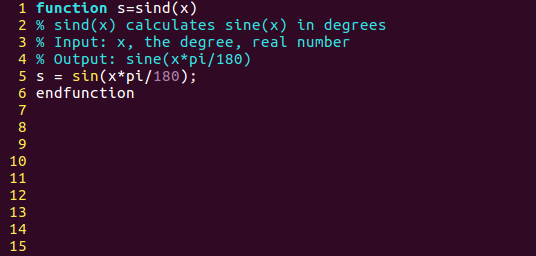
\includegraphics[width=.8\textwidth]{sind.png}
	\end{center}
	\caption{函数示例}
%	\label{fig:<+label+>}
\end{figure}
\begin{itemize}
	\item Line1 该行告诉Octave本文件定义的是一个函数而不是脚本。该行表明定义了一个名为sind的函数,而且该函数接受一个输入参数并返回一个返回值。
	\item Line2,3,4 这几行为注释行,说明了该函数的功能,输入参数以及输出值。和脚本中的一样,函数中这部分注释将被Octave帮助系统识别为有关该函数的说明,并在用户使用 help sind时被返回.
	\item Line5 该行是实现函数的真正功能。它将获取x的值并将计算结果赋给返回值s。
	\item Line6 Octave中函数的结尾需要以endfunction结束。通常Octave不需要return语句(当然你可以使用该语句从函数体中间跳出)来终止函数体。
\end{itemize}
\section{与MATLAB的区别}
 Octave成为一个系统开发项目后,一直试图兼容MATLAB,甚至将这作为一个目标。但是这种兼容不是无原则的模仿。Octave的开发者大多也都是MATLAB的高手,他们实现一个和MATLAB兼容功能的时候,都会充分考虑是否值得实现,以及考虑怎么提高这个功能的性能。特别的,Octave的开发者本着实用的奥卡姆剃刀原则,瞄准可能使用到Octave的研究人员群体,大胆的放弃实现一些MATLAB的功能,确保Octave够用就好。再有,Octave主要运行在类UNIX系统下,兼顾了类UNIX用户的习惯,在某些功能上给出了多种选择(比如注释)。以下是Octave和MATLAB的主要区别。有些是Octave的个性和特性,高于同功能的MATLAB实现的性能。由于MATLAB和Octave都处于开发之中,以下所列的各种不同也许很快就不存在了,请注意。
 \begin{itemize}
	 \item 
1.递加、递减运算符
    Octave支持递加、递减运算符,如x++,y--,这与C风格相同。
	 \item 
2.程序块的结束
    Octave既支持和MATLAB兼容的end关键字,也支持独有的关键字"endblock",如endfunction、endif等。Octave之所以采用这种形式,是觉得MATLAB因为使用同一个end而导致函数结构混乱,分不清函数的层次。
	 \item 
3.注释
    Octave既支持和MATLAB兼容的\%,也支持linux系统通用的\#作为注释的引导符。
	 \item 
4.字符串
    Octave使用“”(双引号)和‘’(单引号)都是可以的。
	\begin{figure}[H]
		\begin{center}
			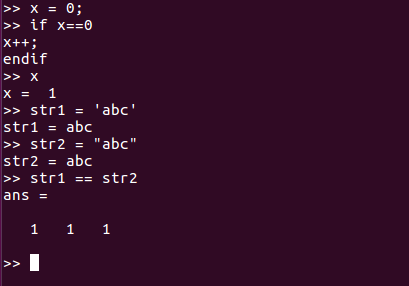
\includegraphics[width=.8\textwidth]{dif1.png}
		\end{center}
	%	\caption{<+caption text+>}
	%	\label{fig:<+label+>}
	\end{figure}
	 \item 
5.函数嵌套
    Octave的作者认为MATLAB的函数嵌套弊大于利,于是在Octave中基本上可以认为不支持嵌套。
	 \item 
6.核心函数
    MATLAB的大部分常用的核心函数(即那些不包含在toolbox中的函数)都已经在Octave中实现了。没有实现的函数,大多是专用于某项功能的函数且这项功能Octave并没有实现(GUI、ActiveX等)。
	 \item 
	 \item 
7.绘图
	Octave的画图后台是强大的Gnuplot,有人认为绝对不会弱于Matlab,而且输出格式要远多于Matlab,公式显示也要强大很多。但也有人说Octave绘图速度比Matlab慢。
	 \item 
8.GUI
    目前,Octave没有实现与MATLAB GUI的兼容。因为Octave的用户大多并不需要一个GUI,或者即使有GUI,他们也不用。所以他们并不怎么对开发一个与MATLAB的GUI类似的东西感兴趣。
	 \item 
9.Simulink
    Octave没有支持Simulink。主要原因是开发人员认为Simulink模型是落后于研究的,并且缺少灵活性,在实际的研究环境中基本不会用到。这也表明了Octave开发者和使用者的群体:主要是面向前沿研究的,需要个性化定制数值计算的工具。
	 \item 
10.工具箱
    Octave是一个社区项目,工具箱都是由爱好者资源提供的。所以在和MATLAB工具箱的兼容性上是不怎么考虑的。
	 \item 
11.函数的书写
    Octave允许在命令行中写函数。这是MATLAB不支持的。
	\item
12.费用方面
	Octave是完全免费的(并且是开源的),而Matlab是商业软件,价格很昂贵(当然,这在当前国情下不是问题)。商业版的优势是有非常完善的服务,即使没有购买正版,也可以在MathWorks官方网站上获得很多非常有价值的资源。
	\item
13.占用空间
	Octave比较小,安装程序只有几十兆;而Matlab非常庞大,最新版的安装程序大约8G,即使只安装最基本的系统,至少也要几百兆以上。Matlab之所以那么庞大,是因为有大量的面向各种应用领域的工具箱,Octave无法相比的。
 \end{itemize}
 \newpage
\section{总结}
这次对Octave的学习,由于其与MATLAB的相似性,一方面可以试做是对MATLAB的基本知识的回顾与总结,另一方面则是对它们的比较。通过学习,我们看到,Octave的大部分操作与MATLAB是兼容的,可以说MATLAB上的指令在Octave上基本都得到了很好的“克隆”。在尽可能兼容MATLAB的同时,Octave的开发者们也注入了他们自己的一些心得,这在某些程度上方便了使用者。但要看到的是,Octave作为一个开源软件,它的安装程序很小,比起有着多年商业使用经验,已经非常成熟的MATLAB来说,还是单薄了些。想要更加全面的功能的话,MATLAB无疑还是首选,而如果使用需求并不大,Octave足以替代MATLAB。
\end{document}

